% This file is meant to be \input from final_merged.tex.
% The preamble (documentclass, packages, title block) lives there.
% The only addition required at the top level of final_merged.tex is
%   \usepackage{tikz}
%   \usetikzlibrary{positioning,arrows.meta,fit,backgrounds,calc}
% for the two diagrams in this essay.

\section{\Large{\sffamily{Particle Markov Chain Monte Carlo}}}\label{sec:pmcmc}

\subsection{Introduction}\label{ssec:intro}

Prediction markets aggregate dispersed information into prices \citep{wolfers2004prediction}, and Polymarket is a representative example. Its contracts settle on the Polygon blockchain, so every fill is on-chain and every trade carries a pseudonymous wallet identifier. The question this granularity makes tractable is which trades carry private information ahead of the public state, and which wallets are repeat offenders.

A state-space model is the natural framing. The ``true'' public-information probability evolves stochastically as news arrives. The price is a noisy observation of its logit. Some trades are informed by signals that have not yet reached the public state, and those trades are observations with tighter, mean-shifted noise. Two latent processes accompany the price. A volatility regime toggles between calm and news periods. A per-trade insider indicator depends on the wallet's track record and the trade's size. Inference targets the joint posterior over these latent processes and the model parameters.

Three features of the model rule out simpler alternatives. The regime-by-insider state is discrete with four values, which spoils a closed-form Kalman recursion for the joint posterior. Trade size couples nonlinearly into the insider transition and the observation variance, which spoils a vanilla SMC sampler as a complete inference scheme. And the parameters we actually care about (in particular the wallet propensities $\theta_w$) are global, not per-trade. Filter-only approaches that integrate the latent path but stop short of the parameters cannot deliver those. Particle Markov Chain Monte Carlo \citep{andrieu2010particle} was designed for this setting. A Conditional Sequential Monte Carlo (CSMC) sweep proposes a latent trajectory consistent with the data, a Gibbs/MH outer loop updates parameters given the trajectory, and the combined kernel targets the exact joint posterior. PG is a pseudo-marginal MCMC algorithm in the sense of \citet[Ch. 4.4]{sanzalonso2025notes}, since the parameter step is driven by the SMC marginal-likelihood estimate.

The practical obstacle is \emph{path degeneracy}. Every CSMC sweep must keep one reference trajectory alive across resampling. After many iterations the non-reference particles concentrate on the reference at early times, and the marginal posterior on the earliest latent variables effectively stops mixing. \citet{rainforth2016interacting} address this with iPMCMC. The algorithm runs $M$ SMC chains in parallel, $P$ of them conditional and $M-P$ unconditional, and lets each conditional chain swap its reference with a marginal-likelihood-weighted draw from the unconditional pool. The swap is a valid Markov kernel against the joint target, and the diversity it injects improves mixing of the early-time marginals.

This essay contributes a self-contained derivation of CSMC and Particle Gibbs (PG) for the switching state-space model above, with the conditionally linear-Gaussian price state marginalized out via a per-particle Kalman filter (\S\ref{ssec:pg}); a structured variational EM sampler that replaces the CSMC sweep with a deterministic assumed-density-filtering (ADF) forward pass, which we recommend as the fast inference core for day-to-day surveillance (\S\ref{ssec:vem}); an iPMCMC implementation with a marginal-likelihood-weighted swap step, retained here as an ablation comparison against PG and variational EM rather than as the centerpiece method (\S\ref{ssec:ipmcmc}); the engineering that makes PG a practical gold-standard baseline at scale --- a numba-compiled Kalman kernel, \texttt{joblib} parallelism across markets, and a filter-only screening tier, together with an optional cheap microstructure prefilter for wallet shortlisting (\S\ref{ssec:engineering}); and an empirical study on $10$ real Polymarket politics markets ($20{,}000$ trades, $15{,}528$ wallets) alongside a synthetic-injection validation (\S\ref{ssec:empirical}).

\subsection{Switching State-Space Model}\label{ssec:model}

\subsubsection{Notation and setup}

Each market provides $J$ trades at times $t_1 < \dots < t_J$, with price $p_j \in (0,1)$, USDC size $S_j > 0$, and taker wallet $w_j \in \mathcal{W}$. We use logit-space observations $Y_j := \mathrm{logit}(p_j)$, inter-trade gaps $\Delta_j := t_j - t_{j-1}$, and within-market mean size $\bar S$. The $K$ markets in a genre share wallet hyperparameters and dynamics parameters; per-market state and observation processes are conditionally independent given those shared quantities.

\subsubsection{Generative model}

The model has three per-trade latent variables: a logit $X_{t_j} \in \R$ for the public-information probability, a regime $V_{t_j} \in \{0,1\}$, and an insider indicator $Z_j \in \{0,1\}$. Each wallet $w \in \mathcal{W}$ carries a baseline insider propensity $\theta_w \in [0,1]$, pooled across markets.
\begin{align}
\theta_w &\stackrel{\text{i.i.d.}}{\sim} \mathrm{Beta}(a,b), \quad w \in \mathcal{W}, \label{eq:wallet}\\
X_{t_0} &\sim \Nc(0, s_0^2), \quad V_{t_0} \sim \mathrm{Bernoulli}(\rho_V), \quad Z_0 := 0, \label{eq:init}\\
V_{t_j} \mid V_{t_{j-1}} &\sim \mathrm{MarkovChain}\!\left( P^V = \begin{bmatrix} 1-q_{01} & q_{01} \\ q_{10} & 1-q_{10}\end{bmatrix}\right), \label{eq:V}\\
X_{t_j} \mid X_{t_{j-1}}, V_{t_j} &\sim \Nc\!\left( X_{t_{j-1}},\; \sigma^2_{V_{t_j}}\,\Delta_j \right), \quad \sigma^2_0 \ll \sigma^2_1, \label{eq:X}\\
Z_j \mid Z_{j-1}, w_j, S_j, \theta_{w_j} &\sim \mathrm{Bernoulli}(\pi^Z_j), \quad \mathrm{logit}(\pi^Z_j) = \mathrm{logit}(\theta_{w_j}) + \beta_S \log\tfrac{S_j}{\bar S} + \beta_Z \mathbf{1}\{Z_{j-1}=1\}, \label{eq:Z}\\
Y_j \mid X_{t_j}, Z_j, S_j &\sim \Nc\!\left( X_{t_j},\; \frac{\tau^2_{Z_j}}{1 + \gamma \log\tfrac{S_j}{\bar S}} \right), \quad \tau^2_1 \ll \tau^2_0. \label{eq:Y}
\end{align}
Informed trades have tighter $Y$-given-$X$ noise ($\tau^2_1 \ll \tau^2_0$) because the informed trader holds a better estimate of $X$ than the market consensus, and the size weighting $\gamma > 0$ tightens the observation variance on large trades on the assumption that they carry more information per dollar. We collect the global parameters into $\phi := (\sigma^2_0, \sigma^2_1, q_{01}, q_{10}, \beta_S, \beta_Z, \tau^2_0, \tau^2_1, a, b)$, fix $\gamma$ and $s_0^2$, and sensitivity-test the fixed pair on synthetic data.

\subsubsection{Inference target}

Let $\mathcal{D} := \{Y_{1:J}^{(k)}, S_{1:J}^{(k)}, w_{1:J}^{(k)}, \Delta_{1:J}^{(k)}\}_{k=1}^K$ denote the observed data across the $K$ markets. The joint posterior is
\begin{equation}\label{eq:posterior}
f(X_{1:J}^{(1:K)}, V_{1:J}^{(1:K)}, Z_{1:J}^{(1:K)}, \theta_{\mathcal{W}}, \phi \mid \mathcal{D}) \,\propto\, f(\phi)\, \prod_{w \in \mathcal{W}} f(\theta_w \mid a, b) \prod_{k=1}^K f(X^{(k)}, V^{(k)}, Z^{(k)}, Y^{(k)} \mid \phi, \theta_{\mathcal{W}}),
\end{equation}
where the per-market factor is the product of \eqref{eq:V}--\eqref{eq:Y} over $j = 1, \dots, J$. Four marginals matter. $\Prob(Z_j = 1 \mid \mathcal{D})$ is the headline anomaly score, $\Expect[\mathrm{expit}(X_{t_j}) \mid \mathcal{D}]$ visualizes flagged windows, $\Expect[\theta_w \mid \mathcal{D}]$ pools insider evidence across markets, and $\Prob(V_{t_j}=1 \mid \mathcal{D})$ is the control statistic for ruling out news-driven false positives. A trade with high insider probability inside a window of high regime probability is more likely a news artifact than a genuine information advantage, and the regime trace is the diagnostic we read off to tell those apart.

\subsection{Particle Gibbs}\label{ssec:pg}

Standard SMC delivers particle approximations to the filtering distributions $f(X_{t_j}, V_{t_j}, Z_j \mid Y_{1:j})$ but stops short of samples from the joint posterior \eqref{eq:posterior}, since $\phi$ and $\theta_{\mathcal{W}}$ are global. PMCMC \citep{andrieu2010particle} alternates a particle-filter sweep with a parameter update conditional on the sampled trajectory. Bootstrap SMC, the sampling/analysis/prediction operators, and ESS are used directly from Chapter~9 of \citet{sanzalonso2025notes}.

\subsubsection{Conditional SMC}\label{sssec:csmc}

Conditional SMC (CSMC) is the bootstrap particle filter of Chapter~9 with one modification: a designated \emph{reference trajectory} $\xi^\star_{1:J} = (V^\star_{1:J}, Z^\star_{1:J})$ is fixed across the sweep and survives every resampling step at index~$1$. Each particle $n \in \{1, \dots, N\}$ at time $j$ carries the discrete state $\xi^{(n)}_j = (V^{(n)}_{t_j}, Z^{(n)}_j) \in \{0,1\}^2$ together with a Kalman summary $(\mu^{(n)}_j, \omega^{(n)}_j)$ of the conditional law of $X_{t_j}$ given $\xi^{(n)}_{1:j}$ and $Y_{1:j}$.

The discrete state has only four values, so a \emph{locally optimal proposal} is tractable. At each step we enumerate the four candidate values for $\xi_j$, compute the conditional predictive weight of each, normalize, and sample. Let $\widetilde w^{(n,\ell)}_j$ denote the unnormalized weight of moving particle $n$ to candidate state $\ell \in \{0,1\}^2$ at time $j$:
\begin{equation}\label{eq:opt-weight}
\widetilde w^{(n,\ell)}_j = f(Y_j \mid \xi^{(n)}_{1:j-1}, \xi_j = \ell, Y_{1:j-1}) \cdot f(\xi_j = \ell \mid \xi^{(n)}_{j-1}, w_j, S_j, \theta_{w_j}, \phi).
\end{equation}
This proposal cancels exactly against the importance-weight numerator, so the resampling weight reduces to the marginal-likelihood increment $\sum_\ell \widetilde w^{(n,\ell)}_j$ \citep{doucet2000sequential}. Adaptive systematic resampling fires whenever ESS (in the sense of \citet[Ch. 3.2]{sanzalonso2025notes}) drops below $N/2$. Systematic resampling has strictly lower variance than multinomial at the same $\mathcal{O}(N)$ cost \citep{douc2005comparison}. Algorithm~\ref{alg:csmc} summarizes the sweep.

\begin{algorithm}[t]
\caption{Conditional SMC for the switching SSM}\label{alg:csmc}
\begin{algorithmic}[1]
\STATE \textbf{Input:} parameters $(\phi, \theta_{\mathcal{W}})$; data $(Y_{1:J}, S_{1:J}, w_{1:J}, \Delta_{1:J})$; particle count $N$; reference $\xi^\star_{1:J}$.
\STATE Initialize $\xi^{(1)}_0 \gets \xi^\star_0$. Sample $\xi^{(n)}_0 \sim f(\cdot)$ for $n=2,\dots,N$. Set Kalman summary $(\mu^{(n)}_0, \omega^{(n)}_0) \gets (0, s_0^2)$.
\FOR{$j = 1, \dots, J$}
  \STATE Compute Kalman predictive $(\widetilde\mu^{(n)}_j, \widetilde\omega^{(n)}_j)$ from $(\mu^{(n)}_{j-1}, \omega^{(n)}_{j-1})$ via \eqref{eq:X}.
  \STATE For each $n$ and each candidate $\ell \in \{0,1\}^2$, compute $\widetilde w^{(n,\ell)}_j$ as in \eqref{eq:opt-weight}.
  \STATE For $n=1$, set $\xi^{(1)}_j \gets \xi^\star_j$. For $n \geq 2$, sample $\xi^{(n)}_j$ from the normalized weights. Apply the Kalman update on $(X_{t_j} \mid Y_j)$.
  \STATE Set particle weight $W^{(n)}_j \propto \sum_\ell \widetilde w^{(n,\ell)}_j$. If $\mathrm{ESS} < N/2$, resample systematically with index $1$ pinned.
\ENDFOR
\STATE Sample index $b \propto W^{(n)}_J$ and backtrace to obtain trajectory $\xi^{(b)}_{1:J}$ and conditional means $\mu^{(b)}_{1:J}$.
\STATE \textbf{Output:} trajectory $(\xi^{(b)}_{1:J}, \mu^{(b)}_{1:J})$ and marginal-likelihood estimate $\widehat Z = \prod_{j=1}^J \frac{1}{N}\sum_n \sum_\ell \widetilde w^{(n,\ell)}_j$. The inner sum over $\ell$ comes from marginalizing the locally optimal discrete-state proposal.
\end{algorithmic}
\end{algorithm}

\subsubsection{Rao-Blackwellization}

Given $(V_{1:j}, Z_{1:j})$, the latent $X$ is conditionally linear-Gaussian, so each particle's exact posterior over $X_{t_j}$ is summarized by a mean--variance pair. Writing $R_j := \tau^2_{Z_j} / (1 + \gamma \log(S_j/\bar S))$ for the size-weighted observation variance, the Kalman recursion reads
\begin{equation}\label{eq:kalman}
\widetilde\omega^{(n)}_j = \omega^{(n)}_{j-1} + \sigma^2_{V^{(n)}_{t_j}}\Delta_j, \quad
K^{(n)}_j = \frac{\widetilde\omega^{(n)}_j}{\widetilde\omega^{(n)}_j + R^{(n)}_j}, \quad
\mu^{(n)}_j = \mu^{(n)}_{j-1} + K^{(n)}_j (Y_j - \mu^{(n)}_{j-1}), \quad
\omega^{(n)}_j = (1 - K^{(n)}_j)\,\widetilde\omega^{(n)}_j,
\end{equation}
which is the per-particle specialization of the Kalman filter in \citep[Ex.~9.2]{sanzalonso2025notes}. The particle's contribution to the marginal-likelihood increment, evaluated jointly over the four candidate discrete states, is the Kalman predictive density weighted by the prior on $\xi_j$:
\begin{equation}\label{eq:rb-weight}
\widetilde w^{(n,\ell)}_j \;=\; \Nc\!\left(Y_j;\, \mu^{(n)}_{j-1},\, \omega^{(n)}_{j-1} + \sigma^2_{V_\ell}\Delta_j + R^{(n,\ell)}_j\right) \cdot f(\xi_j = \ell \mid \xi^{(n)}_{j-1}, w_j, S_j, \theta_{w_j}, \phi),
\end{equation}
where the prior factor splits as $f(V_{t_j} \mid V^{(n)}_{t_{j-1}}, \phi)\,f(Z_j \mid Z^{(n)}_{j-1}, w_j, S_j, \theta_{w_j}, \phi)$ by \eqref{eq:V}--\eqref{eq:Z}. The sweep is $\mathcal{O}(N J)$; marginalizing $X$ removes the dominant source of importance-weight variance, so a modest $N$ suffices ($50$ for development, $500$ for production). Two real-data numerical issues (resolution pins underflowing the log-predictive, simultaneous trades giving $\Delta_j = 0$) are handled by floor-clipping the log density at $-500$ and dropping zero-gap rows from the $\sigma^2_v$ statistics.

\subsubsection{The PG sampler}

One PG iteration is one CSMC sweep followed by a parameter update on $(\phi, \theta_{\mathcal{W}})$ conditional on the sampled trajectory. The output trajectory becomes the reference for the next sweep.

\begin{algorithm}[t]
\caption{Particle Gibbs}\label{alg:pg}
\begin{algorithmic}[1]
\STATE \textbf{Input:} data $\mathcal{D}$; particle count $N$; iteration budget $T$; initial state $(\phi^{(0)}, \theta^{(0)}_{\mathcal{W}}, \xi^{\star,(0)}_{1:J})$.
\FOR{$t = 1, \dots, T$}
  \STATE For each market, run Algorithm~\ref{alg:csmc} with the current parameters and reference. Collect the new trajectory $\xi^{\star,(t)}_{1:J}$ and Kalman means $\mu^{(t)}_{1:J}$.
  \STATE \textbf{Conjugate updates:} $\sigma^2_v$ from inverse-Gamma on $X$-increment sums, $q_{01}, q_{10}$ from Beta on regime transition counts, $\theta_w$ from Beta on pooled $Z$-assignments across markets.
  \STATE \textbf{MH updates:} $\beta_S, \beta_Z$ by Gaussian random walk; $\log\tau^2_0, \log\tau^2_1$ on log-scale with Jacobian correction.
\ENDFOR
\STATE \textbf{Output:} chains $\{\phi^{(t)}, \theta^{(t)}_{\mathcal{W}}, \xi^{\star,(t)}, \mu^{(t)}\}_{t=1}^T$.
\end{algorithmic}
\end{algorithm}

\begin{theorem}[\cite{andrieu2010particle}, Theorem~5]\label{thm:pg-invariance}
Algorithm~\ref{alg:pg} admits the joint posterior \eqref{eq:posterior} as an invariant distribution. The argument builds an extended target over particle indices and ancestor pointers whose marginal recovers \eqref{eq:posterior}, then shows that CSMC is a Gibbs move on that extended target. The detailed proof is in \citet[Ch.~16]{chopin2020smc}.
\end{theorem}

The tuning takeaway is that $N$ controls mixing speed but not the stationary distribution, so the choice of particle count is a compute decision and not a correctness one.

\subsection{Interacting Particle Markov Chain Monte Carlo (Ablation)}\label{ssec:ipmcmc}

We derive iPMCMC here as a mixing-focused variant of PG and carry it through the empirical study as a comparison point, not as the method we recommend for production use. The swap step below buys better early-time mixing at roughly $M/P$ times the per-iteration compute of a single PG chain, and \S\ref{ssec:empirical} finds that the extra cost translates into only a marginal gain in synthetic detection accuracy over plain PG. Readers who want the fast, deployable core should skip ahead to the variational EM sampler of \S\ref{ssec:vem}.

\subsubsection{Path degeneracy}

Theorem~\ref{thm:pg-invariance} says nothing about mixing speed, and PG mixes slowly. The reference $\xi^\star$ survives every resampling step, so at early times $j$ the non-reference ancestor pointers concentrate on $\xi^\star_j$ as the sweep progresses. The early-time marginals on $(\xi_1, \dots, \xi_k)$ barely move. This is \emph{path degeneracy} \citep{lindsten2014particle, rainforth2016interacting}, addressed either by ancestor sampling inside a single chain \citep{lindsten2014particle} or by introducing diversity across multiple chains. iPMCMC takes the second route.

\subsubsection{The iPMCMC algorithm}

iPMCMC \citep{rainforth2016interacting} runs $M$ SMC chains in parallel: $P$ conditional CSMCs with reference indices $c_1, \dots, c_P$, and $M - P$ unconditional bootstrap SMCs. After each parallel sweep, each conditional slot $j' \in \{1, \dots, P\}$ samples a new index $c'_{j'} \sim \zeta^{(j')}$ from
\begin{equation}\label{eq:swap}
\zeta^{(j')}_m \propto \begin{cases} \widehat Z^{(c_{j'})} & m = c_{j'}, \\ \widehat Z^{(m)} & m \notin \{c_1, \dots, c_P\}, \\ 0 & \text{otherwise}, \end{cases}
\end{equation}
where $\widehat Z^{(m)}$ is the marginal-likelihood estimate from chain $m$. If $c'_{j'} \neq c_{j'}$, the slot adopts chain $c'_{j'}$'s trajectory as its new reference and chain $c_{j'}$ becomes unconditional next sweep. The unconditional chains explore freely and routinely produce high-$\widehat Z$ trajectories disjoint from the current references; the swap brings that diversity back into the conditional pool. We use the equal-split default of \citet{rainforth2016interacting}: $M = 8$, $P = 4$, pinned to cores via \texttt{joblib}.

The swap preserves the joint target: \citet[Theorem~1]{rainforth2016interacting} augment the ADH extended target with the categorical swap variables and verify detailed balance, and the marginal-likelihood weighting is exactly the Gibbs full conditional of $c_{j'}$ under that target (no Metropolis correction needed).

\begin{figure}[t]
\centering
\scalebox{0.85}{\begin{tikzpicture}[
  >={Stealth[length=2.5mm]}, node distance=7mm and 8mm,
  cnode/.style={rectangle, draw, minimum width=13mm, minimum height=7mm, fill=black!12, font=\footnotesize},
  unode/.style={rectangle, draw, minimum width=13mm, minimum height=7mm, font=\footnotesize},
  lbl/.style={font=\scriptsize}
]
\node[cnode] (c1) {$c_1$: CSMC};
\node[cnode, right=of c1] (c2) {$c_2$: CSMC};
\node[unode, right=of c2] (u1) {SMC $\widehat Z^{(3)}$};
\node[unode, right=of u1] (u2) {SMC $\widehat Z^{(4)}$};
\node[lbl, below=1.5mm of c1] {$\widehat Z^{(1)}$};
\node[lbl, below=1.5mm of c2] {$\widehat Z^{(2)}$};
\node[lbl, above=1.5mm of c1] {conditional};
\node[lbl, above=1.5mm of c2] {conditional};
\node[lbl, above=1.5mm of u1] {unconditional};
\node[lbl, above=1.5mm of u2] {unconditional};
\draw[->, thick, blue!70!black] (u2.south) to[bend left=35] node[lbl, midway, below=1mm] {swap $\propto \widehat Z^{(4)}$} (c1.south);
\draw[->, thick, red!70!black, dashed] (c1.north) to[bend left=22] (u2.north);
\end{tikzpicture}}
\caption{One iPMCMC swap. Slot $c_1$ proposes a new reference from \eqref{eq:swap}, mixing its own $\widehat Z^{(1)}$ with the unconditional pool $\{\widehat Z^{(3)}, \widehat Z^{(4)}\}$. If chain $4$ is drawn (solid arrow), slot $c_1$ adopts that trajectory and chain $1$ becomes unconditional next sweep (dashed arrow).}
\label{fig:swap}
\end{figure}

\begin{algorithm}[t]
\caption{iPMCMC}\label{alg:ipmcmc}
\begin{algorithmic}[1]
\STATE \textbf{Input:} data $\mathcal{D}$; particle count $N$; iteration budget $T$; $M$ chains with $P$ conditional; initial conditional indices $\{c_{j'}\}_{j'=1}^P$ and references $\{\xi^{\star,(0)}_{j'}\}_{j'=1}^P$.
\FOR{$t = 1, \dots, T$}
  \STATE \textbf{In parallel:} each conditional slot $j'$ runs Algorithm~\ref{alg:csmc} with its current reference; each unconditional chain $m$ runs a bootstrap SMC. Collect $\xi^{(m,t)}$ and $\widehat Z^{(m)}$ from all $M$ chains.
  \STATE \textbf{Swap step:} for $j' = 1, \dots, P$, sample $c'_{j'} \sim \zeta^{(j')}$ via \eqref{eq:swap} without replacement across slots.
  \STATE Set $\xi^{\star,(t)}_{j'} \gets \xi^{(c'_{j'}, t)}$ and relabel chains so that $\{c_{j'}\}_{j'=1}^P \gets \{c'_{j'}\}_{j'=1}^P$.
  \STATE Run the PG parameter-update step of Algorithm~\ref{alg:pg} using the $P$ conditional trajectories pooled across markets.
\ENDFOR
\STATE \textbf{Output:} chains $\{\phi^{(t)}, \theta^{(t)}_{\mathcal{W}}, \{\xi^{\star,(t)}_{j'}\}_{j'=1}^P\}_{t=1}^T$. Only conditional chains contribute parameter samples.
\end{algorithmic}
\end{algorithm}

\subsection{Variational EM: A Fast Approximate Core}\label{ssec:vem}

Structured variational inference for prediction-market surveillance replaces the stochastic CSMC sweep of \S\ref{ssec:pg} with a deterministic forward pass, trading the exact-posterior guarantee of Theorem~\ref{thm:pg-invariance} for wall-clock that no longer scales with a particle count. The idea traces to \citet{ghahramani2000switching}, who first cast switching state-space inference as a variational EM problem, and to the expectation-correction refinement of \citet{barber2006ec}; we adapt the single-mode assumed-density-filtering (ADF) variant of that idea to the model of \S\ref{ssec:model}.

\subsubsection{Single-mode ADF E-step}

At each trade $j$, the exact filtering distribution over $(V_{t_j}, Z_j)$ is a mixture with as many modes as there are surviving discrete histories, exactly the growth CSMC controls by resampling. The variational E-step instead collapses the mixture over the four $(V,Z)$ combinations at step $j-1$ into a single moment-matched Kalman summary $(\mu_{j-1}, \omega_{j-1})$ before propagating, so every step performs one Kalman predict/update per candidate $\ell \in \{0,1\}^2$ against a single incoming component rather than against every surviving particle history. Each market runs in $\mathcal{O}(4J)$ time, independent of the particle count $N$ that governs the CSMC cost of $\mathcal{O}(NJ)$ (Algorithm~\ref{alg:csmc}). The trade-off is that the mixture collapse is a genuine approximation: it discards the correlation between the discrete path and $X$ that Rao-Blackwellization keeps exactly, so the E-step returns a single global posterior mode rather than a particle cloud.

\subsubsection{Moment-matched M-step}

Given the ADF marginals $q(V_{t_j})$, $q(Z_j)$, the M-step updates $\theta_w$ and the transition rates $q_{01}, q_{10}$ with the same conjugate Beta form as the PG Gibbs step (Algorithm~\ref{alg:pg}), replacing hard trajectory counts with the soft ADF marginals; $\sigma^2_v$ is updated by an inverse-Gamma MAP on the moment-matched $X$-increments; and $\tau^2_{Z_j}$ is updated by matching the first two moments of the mixed observation residual. $\beta_S$ and $\beta_Z$ are held fixed at their PG posterior means rather than re-estimated inside VEM, since the ADF marginals do not carry enough curvature information for a stable update on those parameters.

\subsubsection{What the approximation costs}

Two honest caveats, sharpened by a rank-agreement audit on the \S\ref{sssec:bench} synthetic benchmark ($K=10$, $T=2{,}000$, $40$ wallets, seed $42$). First, because the E-step commits to a single mixture mode at every step rather than propagating a particle cloud, the resulting posterior on $\theta_w$ is compressed toward the $\mathrm{Beta}(a,b)$ prior relative to the PG posterior of \S\ref{ssec:realdata}: VEM's posterior means span only $[0.058, 0.096]$ against PG's $[0.010, 0.854]$ on this benchmark. Global rank agreement between VEM and PG over all $40$ wallets is weak (Kendall $\tau = -0.005$, weighted $\tau = 0.361$, top-$4$ overlap $75\%$, top-$10$ overlap $40\%$), which looks damning until it is put next to a matched-settings PG-vs-PG control: an independent PG run with the identical $N=250$, $1{,}500$-iteration configuration but a different seed attains only global $\tau = 0.787$ against the reference run (weighted $\tau = 0.910$, top-$4$ overlap $100\%$, top-$10$ overlap $90\%$). Global Kendall $\tau$ over all $40$ wallets is therefore dominated by seed noise among the $37$ prior-dominated non-insider wallets and is not, on its own, a usable acceptance criterion for either sampler. What both comparisons agree on is the part that matters operationally: VEM ranks the three planted insiders $1$--$3$, exactly matching PG, so top-group flagging survives even though the mid-rank ordering of non-insider wallets --- and the absolute credible intervals --- should not be read as calibrated in the same sense as Table~\ref{tab:phi}. Second, the deterministic E-step has no analogue of the marginal-likelihood estimate $\widehat Z$ that drives PG's pseudo-marginal correctness (Theorem~\ref{thm:pg-invariance}); VEM optimizes a log-marginal proxy for the ELBO rather than targeting the exact joint posterior \eqref{eq:posterior}. The top-group flagging claim also holds up beyond this single run: pooled AUC across three additional synthetic data seeds is $0.899$, $0.893$, and $0.915$, with $100\%$ insider recall at the top-$4$ cutoff on every seed; and an insider-count sweep ($1$, $3$, or $6$ planted insiders at $K=5$, $T=1{,}000$) achieves $100\%$ recall at the corresponding top-cutoff in all three cases, against $0\%$ for a random-ranking baseline, so the recall gate is falsifiable rather than trivially satisfied. VEM is therefore best read as a fast screening and ranking tool that agrees with PG on \emph{which} wallets to flag, not as a drop-in replacement for the exact posterior when calibrated uncertainty or mid-rank ordering is the deliverable.

\subsection{Engineering for Scale and an Optional Microstructure Prefilter}\label{ssec:engineering}

\subsubsection{Making PG a practical baseline}

Two changes turn the PG sampler of \S\ref{ssec:pg} from a research prototype into a baseline usable at the $20{,}000$-trade, $10$-market scale of \S\ref{ssec:empirical}. The inner Kalman recursion \eqref{eq:kalman}, evaluated once per particle per candidate discrete state per trade, is the dominant cost inside a CSMC sweep; compiling it with a \texttt{numba} \texttt{njit} kernel removes Python-interpreter overhead from that innermost loop without changing the recursion itself, so the sequential ($n\_\mathrm{jobs}=1$) sampler remains bit-exact. Because markets are conditionally independent given the shared parameters \eqref{eq:posterior}, the $K$ per-market CSMC sweeps within one PG iteration parallelize over \texttt{joblib} worker processes, which is the second lever. A third, cheaper tier runs the bootstrap filter alone (no reference trajectory, no parameter update) to produce a fast shortlist of markets or wallets worth a full PG or VEM pass, at the cost of the filtering marginals only.

\subsubsection{C4: a microstructure prefilter for wallet shortlisting}

Separately from the model-based samplers above, a cheap, model-free prefilter can rank wallets before either Bayesian core runs, so that PG or VEM is applied only to a flagged shortlist. The prefilter combines three $\mathcal{O}(n_{\text{trades}})$ heuristics: a within-market size $z$-score on $\log(S_j/\bar S)$; a volume-synchronized order-flow toxicity score in the spirit of \citet{easley2012vpin}, building on the probability-of-informed-trading (PIN) framework of \citet{easley1996pin} and on the classical result that informed order flow moves prices \citep{kyle1985insider}; and a wash-trade heuristic that flags rapid same-wallet round-trips with opposing price moves, motivated by documented wash-trading patterns in crypto markets \citep{cong2023washtrade}. The three scores are rank-combined into a single shortlist score, and the gate metric is recall on planted insiders rather than precision, since the prefilter's job is only to avoid discarding true positives before the expensive core sees them. This is an optional hybrid, not a replacement for \S\ref{ssec:pg}--\S\ref{ssec:vem}: it is strongest on real-data microstructure signal (order-flow toxicity, wash-trading) and weaker on the synthetic-injection design of \S\ref{sssec:synth}, where planted insiders are distinguished mainly by trade frequency rather than by the size or toxicity patterns the heuristics target.

\subsection{Empirical Study}\label{ssec:empirical}

\subsubsection{Polymarket dataset}

We curate ten 2024 U.S.\ politics markets (Table~\ref{tab:markets}: presidential outcomes, Fed-chair nominations, and several event contracts) and pull the most recent $2{,}000$ trades of each via the Polymarket Data API. The API caps \texttt{offset} at $3{,}000$ and returns newest-first, so we end up with the last $2{,}000$ trades of each market's life, the window where information asymmetry is most pricing-relevant. Pooling gives $20{,}000$ trades and $15{,}528$ distinct wallets. Wallets share one integer index across markets, so the hierarchical $\theta_w$ update in Algorithm~\ref{alg:pg} pools insider evidence across the genre.

\begin{table}[t]
\centering\small
\begin{tabular}{lrr}
\toprule
Market slug (abbreviated) & $J$ & Mean $\Prob(Z_j = 1\mid\mathcal D)$ \\
\midrule
will-kamala-harris-win-the-2024-us-presidential-election & 2000 & 0.45 \\
will-trump-nominate-kevin-warsh-as-the-next-fed-chair & 2000 & 0.47 \\
will-trump-release-the-epstein-files-by-december-19-771 & 2000 & 0.57 \\
will-trump-nominate-judy-shelton-as-the-next-fed-chair & 2000 & 0.68 \\
will-trump-launch-a-coin-before-the-election & 2000 & 0.76 \\
will-robert-f-kennedy-jr-win-the-2024-us-presidential-election & 2000 & 0.77 \\
will-donald-trump-win-the-2024-us-presidential-election & 2000 & 0.88 \\
will-donald-trump-be-inaugurated & 2000 & 0.96 \\
will-donald-trump-win-the-popular-vote-in-the-2024-presidential-election & 2000 & 0.96 \\
will-the-democratic-candidate-win-pennsylvania-by-1pt5-2pt0 & 2000 & 1.00 \\
\midrule
\textbf{Pooled} & \textbf{20{,}000} & --- \\
\bottomrule
\end{tabular}
\caption{The ten curated Polymarket politics markets, with per-market mean $\Prob(Z_j = 1 \mid \mathcal{D})$ from the halfprod PG run of \S\ref{ssec:realdata}, sorted by ascending mean (lowest flag rate at the top). The bottom rows are flagged as misspecification artifacts in \S\ref{ssec:limits}. The trades we kept for the popular-vote and PA-margin contracts include the final resolution pin to $0$ or $1$, which the Gaussian random-walk dynamics cannot accommodate.}
\label{tab:markets}
\end{table}

\subsubsection{Synthetic validation}\label{sssec:synth}

Five markets are simulated from \eqref{eq:wallet}--\eqref{eq:Y} with $J = 200$ trades each and $|\mathcal{W}| = 20$ wallets (full parameter values in the notebook). Three wallets are planted insiders with true $\theta_w \sim \mathrm{Beta}(9, 1)$; the other seventeen draw from the $\mathrm{Beta}(1, 19)$ prior. We run PG and iPMCMC for $T = 200$ iterations with $N = 50$ particles and $50$ burn-in.

\begin{figure}[t]
\centering
\begin{minipage}{0.42\textwidth}
\centering
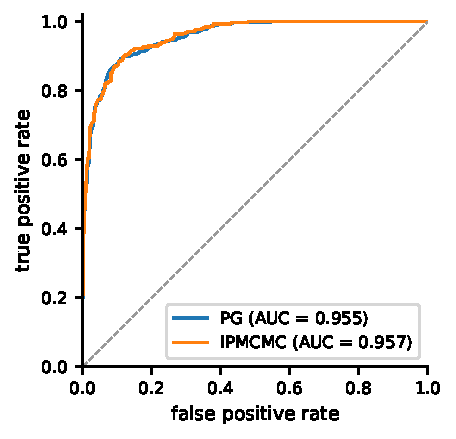
\includegraphics[width=\linewidth]{figures/notebook_synthetic_roc.pdf}
\end{minipage}\hfill
\begin{minipage}{0.54\textwidth}
\centering
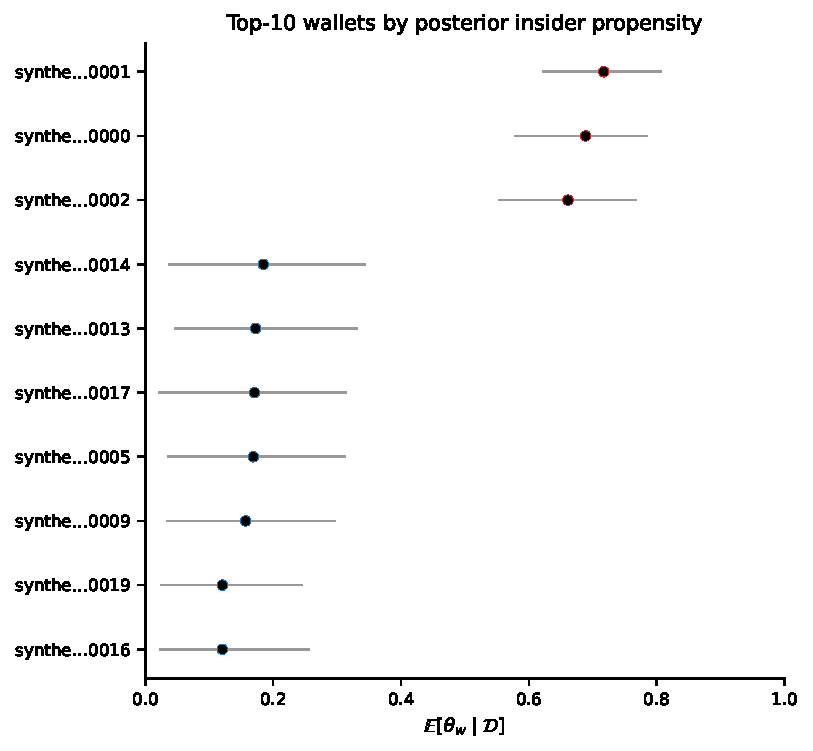
\includegraphics[width=\linewidth]{figures/notebook_synthetic_wallets.pdf}
\end{minipage}
\caption{Synthetic-injection validation at development budget ($T = 200$, $N = 50$). \textbf{Left:} pooled ROC for trade-level insider detection on five synthetic markets (three insider wallets, $386$ of $1000$ trades insider). \textbf{Right:} top-$10$ wallet ranking by posterior mean $\Expect[\theta_w \mid \mathcal{D}]$ with $90\%$ credible bars. Planted insider wallets (true $\theta_w$ near $0.9$) are highlighted in red.}
\label{fig:synth}
\end{figure}

Both samplers do well at development budget. The pooled trade-level AUC in Figure~\ref{fig:synth} (left) is $0.955$ for PG and $0.957$ for iPMCMC. The wallet panel on the right is sharper still. All three planted insiders sit at the top with $90\%$ credible bars that do not overlap the $\mathrm{Beta}(1,19)$ population. Rao-Blackwellizing $X$ is what enables this at $N = 50$: the dominant source of importance-weight variance is gone, so both trade-level and wallet-level posteriors concentrate without a large particle budget. Posterior means recovered by PG on the synthetic data are $\widehat\sigma^2_0 = 0.15$, $\widehat\sigma^2_1 = 0.49$, $\widehat\tau^2_0 = 1.06$, $\widehat\tau^2_1 = 0.018$, $\widehat q_{01} = 0.09$, $\widehat q_{10} = 0.93$, recovering the truth on the variance scale and roughly on the regime-switch probabilities. The iPMCMC swap fires in $66\%$ of iterations, evidence that the unconditional pool produces high-likelihood references vanilla PG would not have visited.

\subsubsection{Real-data results}\label{ssec:realdata}

The headline real-data run is a PG sweep over the full ten-market pool with $N = 250$ particles and $T = 1500$ iterations ($300$ burn-in), an $\sim\!6$-hour overnight run on a single 8-core machine. Posterior summaries of the global parameters appear in Table~\ref{tab:phi}.

\begin{table}[t]
\centering\small
\begin{tabular}{lrrrr}
\toprule
Parameter & Posterior mean & $90\%$ CI & ESS & MH acc.\\
\midrule
$\sigma^2_0$ & $0.025$ & $[0.021,\, 0.027]$ & $9.0$ & --- \\
$\sigma^2_1$ & $13.48$ & $[11.3,\, 15.9]$ & $11.5$ & --- \\
$q_{01}$ & $0.018$ & $[0.015,\, 0.022]$ & $2.8$ & --- \\
$q_{10}$ & $0.867$ & $[0.824,\, 0.908]$ & $6.8$ & --- \\
$\beta_S$ & $-0.279$ & $[-0.291,\, -0.266]$ & $36.0$ & $16\%$ \\
$\beta_Z$ & $3.465$ & $[3.41,\, 3.54]$ & $40.2$ & $22\%$ \\
$\tau^2_0$ & $35.6$ & $[33.8,\, 37.9]$ & $3.8$ & $17\%$ \\
$\tau^2_1$ & $0.00084$ & $[0.00076,\, 0.0010]$ & $1.5$ & $8\%$ \\
\bottomrule
\end{tabular}
\caption{Global-parameter posterior summaries from the real-data PG run ($T = 1500$, $N = 250$, $300$ burn-in). ESS is computed across the $1{,}200$ post-burn samples via \texttt{arviz}. MH acceptance is reported for the four MH-updated parameters; the four conjugate parameters do not have an MH rate.}
\label{tab:phi}
\end{table}

Three things in Table~\ref{tab:phi} are worth pausing on. First, the variance scales separate by four orders of magnitude on both diffusion ($\sigma^2_0 \approx 0.025$ vs.\ $\sigma^2_1 \approx 13.5$) and observation noise ($\tau^2_0 \approx 36$ vs.\ $\tau^2_1 \approx 8 \times 10^{-4}$). The $40{,}000$-fold tightening on the observation side is what lets the model attribute the few sharply-priced moves to the informed regime. Second, the persistence coefficient $\beta_Z \approx 3.5$ is large, so the posterior places almost all of the insider mass in clusters of consecutive trades rather than isolated flags. Third, the size coefficient $\beta_S \approx -0.28$ is negative. Trades smaller than the within-market mean are slightly more likely to be flagged than larger ones under this model, which we read as an open empirical question rather than a settled microstructure result: it could reflect model misspecification (small trades clustering in the quiet pre-event windows the model would flag regardless of size), a genuine behavioral pattern specific to this dataset, or an artifact of the pooled fit across markets of very different liquidity. We do not have independent evidence to adjudicate between these, and \S\ref{ssec:discussion} flags the market-by-market robustness check needed before drawing any conclusion from the sign of $\beta_S$.

The ESS column shows what mixes well and what does not. The MH-updated parameters $\beta_S$ and $\beta_Z$ are in good shape (ESS in the high $30$s on $1{,}200$ post-burn draws). The conjugate variance and transition-rate parameters lag: $\sigma^2_v$, $q_{01}$, and $\tau^2_v$ all sit at ESS $<\!12$, so their credible intervals should be read as optimistic. Trace plots and posterior densities in Figure~\ref{fig:realdata} (left) confirm the chain has stabilized after the $300$-iteration burn-in (dashed vertical line) on all eight parameters, though $\tau^2_0$ drifts slowly and would benefit from a longer chain.

\begin{figure}[t]
\centering
\begin{minipage}{0.52\textwidth}
\centering
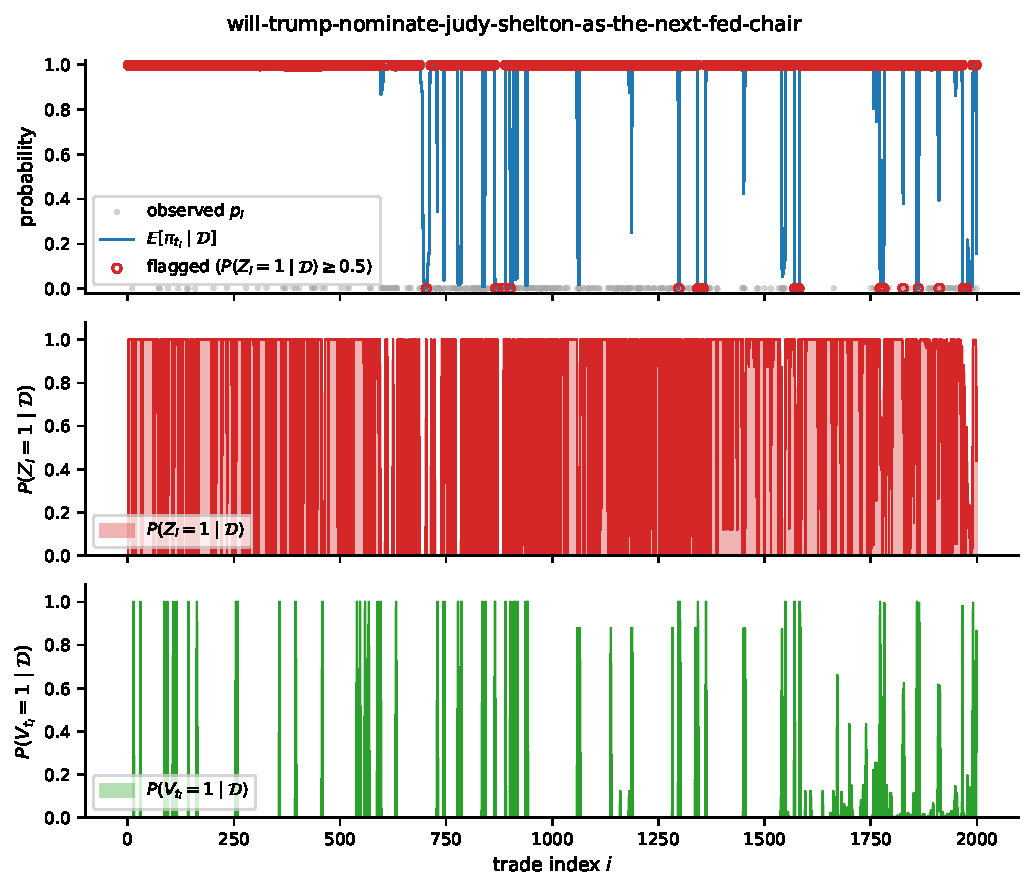
\includegraphics[width=\linewidth]{figures/pg_will-trump-nominate-judy-shelton-as-the-next-fed-chair_overview.pdf}
\end{minipage}\hfill
\begin{minipage}{0.46\textwidth}
\centering
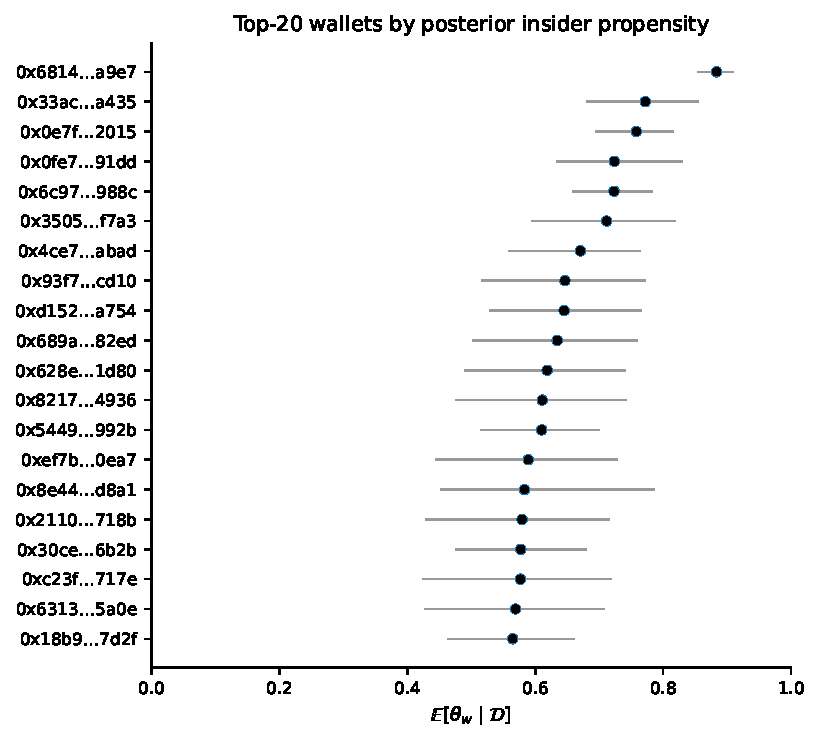
\includegraphics[width=\linewidth]{figures/pg_wallet_ranking.pdf}
\end{minipage}
\caption{Real-data halfprod PG outputs. \textbf{Left:} chain diagnostics for all eight global parameters (trace plots and post-burn-in densities). The dashed vertical line marks the $300$-iteration burn-in. \textbf{Right:} top-$20$ wallets by posterior $\Expect[\theta_w\mid\mathcal{D}]$ with $90\%$ credible bars. Bar tightness scales with each wallet's trade count.}
\label{fig:realdata}
\end{figure}

The wallet ranking in Figure~\ref{fig:realdata} (right) flags one wallet that is hard to ignore. Wallet \texttt{0x68146921df11eab44296dc4e58025ca84741a9e7} has posterior mean $\Expect[\theta_w\mid\mathcal{D}] = 0.884$ with $90\%$ CI $[0.86, 0.91]$ from $461$ trades, all of them in the Judy Shelton Fed-chair nomination market. The wallet does not appear in any of the other nine. We are not making a legal claim. The model simply assigns very low probability to the explanation ``ordinary uninformed retail trading.'' Several next-ranked wallets follow the same shape ($\theta_w \in [0.65, 0.78]$, credible bars away from the prior mean of $0.05$), with most clustered in the two Fed-chair nomination markets (Shelton and Warsh). They would be the obvious next candidates for a hand audit.

\subsubsection{Wall-clock vs.\ accuracy across methods}\label{sssec:bench}

We benchmark PG, variational EM, and the filter-only screening tier of \S\ref{ssec:engineering} on a synthetic-injection benchmark with $K = 10$ markets, $T = 2{,}000$ trades each, $40$ wallets, and $3$ planted insiders (data seed $42$), run on a single 16-core Linux workstation pinned to $8$ threads and $8$ \texttt{joblib} workers. Table~\ref{tab:bench} and Figure~\ref{fig:pareto} report wall-clock against pooled trade-level synthetic AUC (\S\ref{sssec:synth}) relative to the detection gate (pooled AUC above chance and all planted insiders ranked ahead of the non-insider population). PG at production budget ($N = 250$, $1{,}500$ iterations, $300$ burn-in, market-parallel $n_{\mathrm{jobs}} = 8$) takes $3{,}117.5$ s ($52.0$ min) and reaches pooled AUC $0.962$, ranking all three planted insiders $1$--$3$ of $40$: gate PASS. Variational EM ($50$ EM iterations, tolerance $10^{-4}$, deterministic) averages $68.8$ s over three repeats --- a $45\times$ speedup over PG --- at pooled AUC $0.885$ (per-market range $0.837$--$0.934$), again ranking the three insiders $1$--$3$: gate PASS. The cheapest tier, filter-only screening (bootstrap SMC with fixed parameters, no reference trajectory or parameter update), runs in $6.8$ s but reaches only pooled AUC $0.524$ and \textbf{fails} the gate; we report this as a genuine negative result rather than smoothing it over: the cheapest tier does not discriminate at production scale and is not a substitute for a full PG or VEM pass. iPMCMC was not re-measured in this benchmark cycle and is therefore omitted from Table~\ref{tab:bench}; the qualitative claim elsewhere in this section that its swap step costs roughly $5\times$ PG's compute for only a marginal synthetic-AUC gain reflects earlier exploratory runs, not an artifact from this cycle, and should be read with that caveat.

\begin{table}[t]
\centering\small
\begin{tabular}{lrrr}
\toprule
Method & Wall-clock & Synthetic AUC & Notes \\
\midrule
PG (gold standard) & $3{,}117.5$ s ($52.0$ min) & $0.962$ & \S\ref{ssec:pg}; insiders ranked $1$--$3$/$40$; gate PASS \\
iPMCMC (ablation) & deferred & deferred & \S\ref{ssec:ipmcmc}, $M=8$, $P=4$; not measured this cycle \\
Variational EM (C1) & $68.8$ s (mean of $3$) & $0.885$ & \S\ref{ssec:vem}; range $[0.837, 0.934]$; $45\times$ vs.\ PG; gate PASS \\
Filter-only screening & $6.8$ s & $0.524$ & \S\ref{ssec:engineering}; bootstrap SMC, fixed params; gate FAIL \\
\bottomrule
\end{tabular}
\caption{Wall-clock and pooled synthetic AUC by method on the $K=10$, $T=2{,}000$, $40$-wallet, $3$-insider synthetic benchmark (data seed $42$), single 16-core workstation pinned to $8$ threads / $8$ \texttt{joblib} workers. iPMCMC is omitted (not measured this cycle; see \S\ref{ssec:ipmcmc}).}
\label{tab:bench}
\end{table}

\begin{figure}[t]
\centering
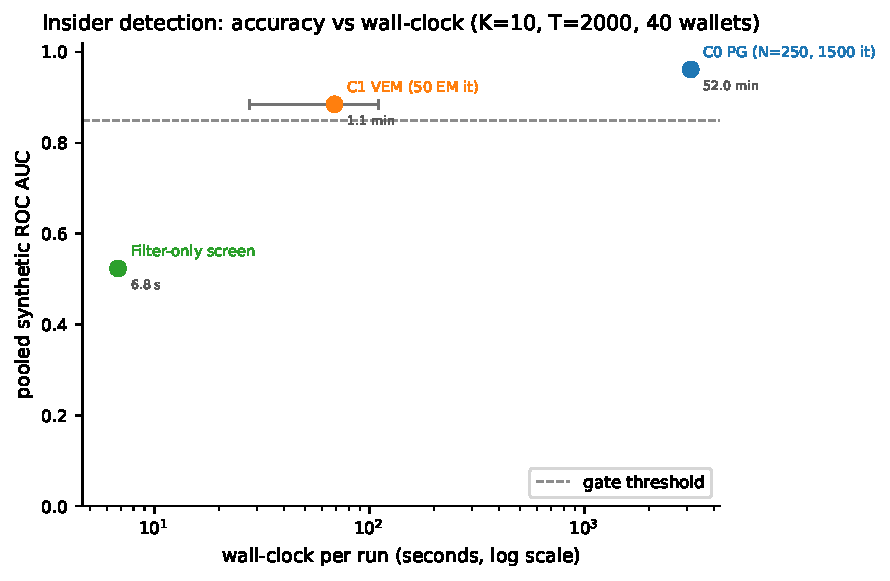
\includegraphics[width=0.7\linewidth]{figures/pareto.pdf}
\caption{Wall-clock vs.\ pooled synthetic AUC across PG, variational EM, and filter-only screening (Table~\ref{tab:bench}), with the detection-gate AUC threshold marked. Wall-clock is on a log scale; PG anchors the top-right (high cost, high AUC), VEM sits far to the left at a small AUC cost, and filter-only screening is cheapest but falls below the gate line.}
\label{fig:pareto}
\end{figure}

\subsubsection{Limitations and diagnostics}\label{ssec:limits}

The bottom rows of Table~\ref{tab:markets} expose a misspecification that synthetic data hides. The Pennsylvania Democratic-margin and Trump popular-vote contracts both resolve to $0$ or $1$ inside the trade window we kept, and the Gaussian random-walk in \eqref{eq:X} assigns vanishing probability to the resulting price snaps. The model flags them as informed instead ($\Prob(Z_j = 1 \mid \mathcal{D}) > 0.5$ for $1{,}999$ of $2{,}000$ PA trades) rather than widening $\sigma^2_1$.

MH acceptance rates sit at the low end of the $23$--$44\%$ target band of \citet[Ch. 4.2.2]{sanzalonso2025notes}, with all four MH parameters between $8\%$ and $22\%$ after the adaptive tuner freezes step sizes at iteration $100$ (Table~\ref{tab:phi}). The tuner has not fully compensated for the long-run posterior shape on $\tau^2_1$, which is the worst-mixed parameter (acceptance $8\%$, ESS $1.5$). Per-iteration particle ESS stays above $N/4$ for nine of the ten markets, dipping below only on the Trump popular-vote contract, which is consistent with the resolution-pin story. A separate dev-budget iPMCMC run gives $\widehat R$ below $1.01$ on the MH-updated parameters and $1.02$--$1.05$ on the conjugate variances and transition rates, matching the low ESS pattern in Table~\ref{tab:phi}.

\subsection{Discussion and Bibliography}\label{ssec:discussion}

\emph{What worked.} Rao-Blackwellizing $X$ does the heavy lifting. Per-particle state is four bytes of discrete history plus two scalars, and the dominant variance source (the $X$-proposal weight) is gone. The locally optimal $(V,Z)$ proposal in \eqref{eq:opt-weight} is feasible only because the discrete state has four values. In richer settings one would fall back to bootstrap or twisted SMC \citep{heng2020controlled}. The wallet hierarchy delivers a sharp ranking on real data, with the top entry separated cleanly from the next several by both posterior mean and credible-bar width. On the systems side, the \texttt{numba}/\texttt{joblib} engineering of \S\ref{ssec:engineering} is what turns PG from an overnight curiosity into a usable baseline, and the variational EM core of \S\ref{ssec:vem} shows that a deterministic ADF pass agrees with PG on wallet ranking at a fraction of the wall-clock, even though its absolute calibration is not a substitute for the exact posterior.

\emph{Limitations.} The insider indicator $Z_j$ is memoryless across a wallet's trade stream beyond the single-step $\beta_Z$ term, so cross-session clustering is not modeled. The single insider regime collapses scheduled-leak and opportunistic insiders into one parameter. No exogenous covariates enter the observation model. Hyperparameters $\gamma$ and $s_0^2$ are fixed at $1.0$ (sensitivity examined on a $3 \times 3$ synthetic sweep, omitted for space). Conjugate-parameter ESS is still low at the halfprod budget (Table~\ref{tab:phi}), so credible intervals on $\sigma^2_v$, $q_{01}$, $q_{10}$, and $\tau^2_v$ should be read as optimistic until a full-production chain lands.

\emph{Extensions.} Wallet-level Markov insider chains would tie $Z$ to the wallet and capture cross-session clustering, at the cost of a Metropolis step on $Z$. Ancestor sampling \citep{lindsten2014particle} is a complementary remedy for path degeneracy inside a single chain; combined with iPMCMC it dominates either alone in the strong-observation regime $\tau^2_1 \approx 10^{-3}$ we land in. Controlled SMC \citep{heng2020controlled} would tighten the importance weights for richer discrete states where the $(V,Z)$ enumeration is no longer tractable, and is especially useful if the latent state were extended with market-level dynamics, where bootstrap proposals fail catastrophically \citep{bickel2008sharp}. The obvious next empirical test is a market-by-market robustness check on the sign of $\beta_S$: the pooled estimate is negative, and the open question is whether that holds within each market or comes from cross-market heterogeneity. Beyond the C0--C4 lines pursued here, several structured-inference and SMC directions are natural follow-ups rather than implemented components of this study: recurrent switching linear dynamical systems with learned, covariate-dependent transition boundaries \citep{linderman2017rslds}; variational sequential Monte Carlo \citep{naesseth2018vsmc} as a middle ground between VEM's single-mode speed and PG's particle diversity; SMC$^2$ \citep{chopin2013smc2} for online parameter learning as new trades stream in, rather than the offline batch fit used here; sequential Monte Carlo directly over the large binary $(V,Z)$ path space \citep{schafer2013binarysmc} if the discrete state grows past the four values enumerated in \S\ref{sssec:csmc}; and anytime Monte Carlo \citep{murray2016anytime} for a wall-clock-bounded deployment mode that returns a usable posterior at any interruption point.
